\documentclass[12pt]{article}
\usepackage{OSUDissertation}

\begin{document}

\setlength{\abovedisplayskip}{5pt}
\setlength{\belowdisplayskip}{5pt}

%%%%%%%%%%%%%%%%%%%%%%%%%%%%%%%%%%%%%%%
\section{\RZ\ Geometry}
\label{sec:RZ}

Solving the transport equation in different coordinate systems may provide simpler ways of modeling a particular geometry or symmetry. In this section, we derive the \RZ\ transport equation to be solved. It assumes there is no variation in the azimuthal direction (of a cylinder), hence problems in \RZ\ geometry look very similar to problems in \XY\ geometry. The streaming operator in cylindrical geometry is \cite{Lewis_Comp_Methods_Neu_Trans}
\begin{flalign}
\vec{\Omega} \vd \grad \psi & = \frac{\mu}{r} \frac{\partial}{\partial r} (r \psi) + \frac{\eta}{r} \frac{\partial \psi}{\partial \zeta} + \xi \frac{\partial \psi}{\partial z} - \frac{1}{r} \frac{\partial}{\partial \omega} (\eta \psi),
\end{flalign}
%
where $\vec{\Omega}$ is the direction of travel unit vector, $\psi$ is the angular flux, and
\begin{flalign}
\mu & \equiv \vec{\Omega} \vd \hat{e}_r = \sqrt{1 - \xi^2} \cos \omega = \sin(\theta) \cos(\omega), \\
\eta & \equiv \vec{\Omega} \vd \hat{e}_\theta = \sqrt{1 - \xi^2} \sin \omega = \sin(\theta) \sin(\omega), \\
\xi & \equiv \vec{\Omega} \vd \hat{e}_z = \cos(\theta).
\end{flalign}
%
The variables $\mu$, $\eta$, $\xi$, $\omega$, and $\theta$ are shown in the cylindrical coordinate system in Figure \ref{fig:CylindricalCoordinateSystem}. We assume there is no solution variation in the azimuthal direction, i.e.
\begin{flalign}
\frac{\partial \psi}{\partial \zeta} & \equiv 0,
\end{flalign}
%
which simplifies the streaming term to
\begin{flalign}
\vec{\Omega} \vd \grad \psi & = \frac{\mu}{r} \frac{\partial}{\partial r} (r \psi) + \xi \frac{\partial \psi}{\partial z} - \frac{1}{r} \frac{\partial}{\partial \omega} (\eta \psi).
\end{flalign}

\begin{figure}[!h]
\tdplotsetmaincoords{60}{110}
\begin{tikzpicture}[scale=10,tdplot_main_coords]
\pgfmathsetmacro{\rvec}{.8}
\pgfmathsetmacro{\phivec}{40}
\pgfmathsetmacro{\thetavec}{50}
\pgfmathsetmacro{\omegavec}{60}

\coordinate (O) at (0,0,0);
\draw[thick,->] (0,0,0) -- (1,0,0) node[anchor=north east]{$x$};
\draw[thick,->] (0,0,0) -- (0,1,0) node[anchor=north west]{$y$};
\draw[thick,->] (0,0,0) -- (0,0,1) node[anchor=south]{$z$};
\tdplotsetcoord{P}{\rvec}{\phivec}{\thetavec}
\draw[-stealth,color=red] (O) -- (P) node[above left] {$(r,z)$};
\draw[dashed, color=red] (O) -- (Pxy);
\draw[dashed, color=red] (P) -- (Pxy);
\tdplotdrawarc[color=red,->]{(O)}{0.2}{0}{\thetavec}{anchor=north}{$\zeta$}

\coordinate (er) at ($(P)+0.4*({cos(\thetavec)},{sin(\thetavec)},0)$);
\coordinate (etheta) at ($(P)+0.4*({-cos(90-\thetavec)},{sin(90-\thetavec)},0)$);
\coordinate (ez) at ($(P)+0.4*(0,0,1)$);
\draw[-stealth] (P) -- (er) node[below right] {$\hat{e}_r$};
\draw[-stealth] (P) -- (etheta) node[below right] {$\hat{e}_\theta$};
\draw[-stealth] (P) -- (ez) node[right] {$\hat{e}_z$};

\coordinate (Omega) at ($(P)+0.2*(-.5,1.5,2)$);
\draw[-stealth,color=blue] (P) -- (Omega) node[above right] {$\vec{\Omega}$};
\draw[dashed,color=blue] (Omega) -- ($(Omega)+0.2*(0,0,-2)$) -- (P);
\tdplotdrawarc[color=blue,->]{(P)}{0.2}{\thetavec}{\thetavec+\omegavec}{anchor=north}{$\omega$}

\tdplotsetthetaplanecoords{\phivec}
\tdplotsetrotatedcoords{\thetavec}{270}{0}
\tdplotsetrotatedcoordsorigin{(P)}
\tdplotdrawarc[tdplot_rotated_coords,color=blue,->]{(0,0,0)}{0.2}{0}{\thetavec}{anchor=south west}{$\theta$}

\end{tikzpicture}
\caption{Cylindrical space-angle coordinate system showing the position $(r,z)$ and direction of travel $\vec{\Omega}$.}
\label{fig:CylindricalCoordinateSystem}
\end{figure}

The transport equation in \RZ\ geometry is then
\begin{multline}
\frac{\mu}{r} \frac{\partial}{\partial r} r \psi \left(r,z, \vec{\Omega} \right) + \xi \frac{\partial}{\partial z} \psi \left(r,z,\vec{\Omega} \right) - \frac{1}{r} \frac{\partial}{\partial \omega} \eta \psi \left(r,z, \vec{\Omega} \right) + \sigma_t \left(r,z \right) \psi \left(r,z,\vec{\Omega} \right) \\
= \frac{1}{4 \pi} \int_{4 \pi} \sigma_s \left(r,z \right) I \left(r,z, \vec{\Omega}^\prime \right) d \Omega^\prime + S_0 \left(r,z, \vec{\Omega} \right)
\label{eq:RZTransport}
\end{multline}

\noindent where $\sigma_t$ is the total cross section, $\sigma_s$ is the scattering cross section, and $S_0$ is an isotropic source as before.

%%%%%%%%%%%%%%%%%%%%%%%%%%%%%%%%%%%%%%%
\subsection{Angular Discretization}
Discretizing Equation \ref{eq:RZTransport} with a level-symmetric angular quadrature results in 
\begin{multline}
\frac{\mu_{n,m}}{r} \frac{\partial}{\partial r} r \psi_{n,m} \left(r,z \right) + \xi_n \frac{\partial}{\partial z} \psi_{n,m} \left(r,z \right) - \frac{1}{r} \frac{\partial}{\partial \omega} \eta_{n,m} \psi_{n,m} \left(r,z \right) + \sigma_t \left(r,z \right) \psi_{n,m} \left(r,z \right) \\
= \frac{1}{4 \pi} \int_{4 \pi} \sigma_s \left(r,z \right) I \left(r,z, \vec{\Omega}^\prime \right) d \Omega^\prime + S_0 \left(r,z, \vec{\Omega} \right)
\label{eq:RZSNTransport}
\end{multline}

\noindent for direction $\vec{\Omega}_{n,m}$, where index $n$ describes a level of quadrature with constant $\xi$ and the $m$ index denotes the quadrature point on that level. The $(n,m)$ indexing is shown in Figure \ref{fig:AngularDiscretization}.

\begin{figure}[!htb]
\centering
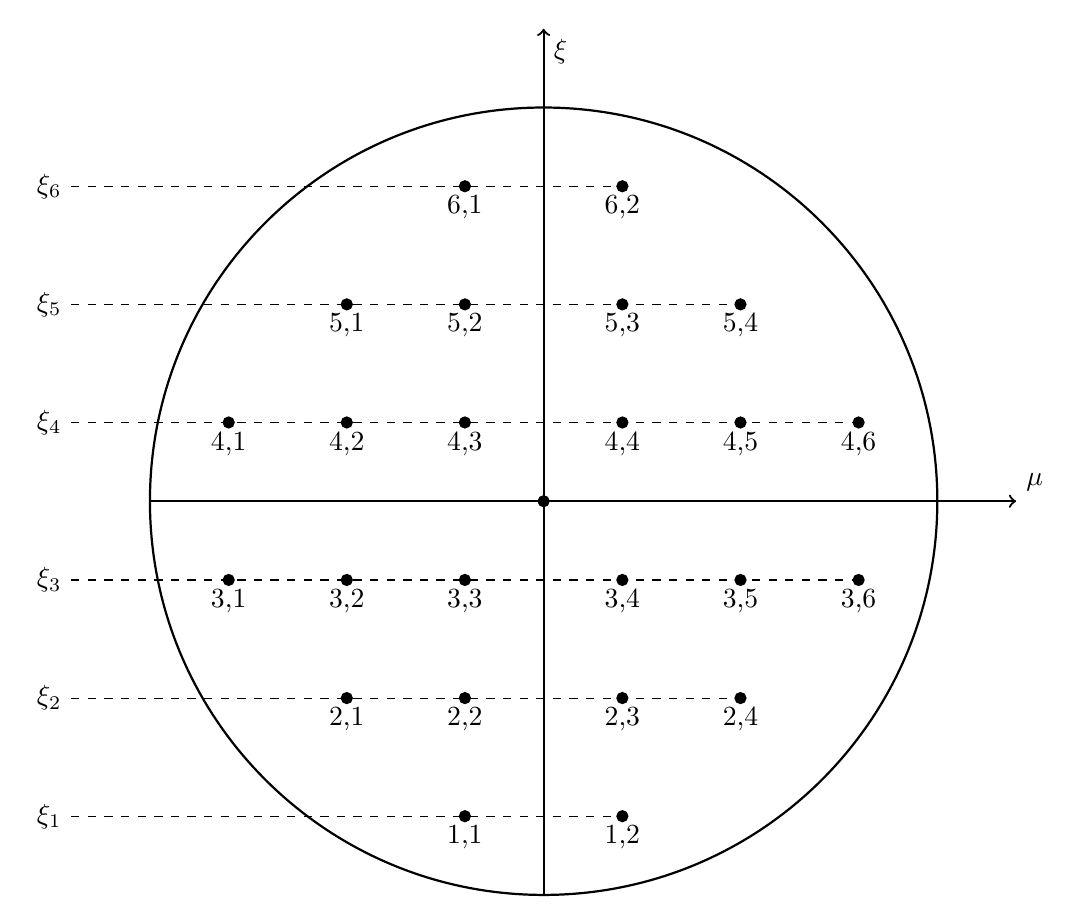
\begin{tikzpicture}

\draw[fill=black] (0,0) circle (2pt);
\draw[thick,->] (-5,0) -- (6,0) node[above right]{$\mu$};
\draw[thick,->] (0,-5) -- (0,6) node[below right]{$\xi$};
\draw[thick] (0,0) circle (5cm);

\draw[dashed] (-6,-4) node[left]{$\xi_1$} -- (1,-4);
\draw[dashed] (-6,-2.5) node[left]{$\xi_2$} -- (2.5,-2.5);
\draw[dashed] (-6,-1) node[left]{$\xi_3$} -- (4,-1);
\draw[dashed] (-6,1) node[left]{$\xi_4$} -- (4,1);
\draw[dashed] (-6,2.5) node[left]{$\xi_5$} -- (2.5,2.5);
\draw[dashed] (-6,4) node[left]{$\xi_6$} -- (1,4);

\draw[fill=black] (-4,-1) circle (2pt) node[below]{3,1};
\draw[fill=black] (-2.5,-1) circle (2pt) node[below]{3,2};
\draw[fill=black] (-1,-1) circle (2pt) node[below]{3,3};
\draw[fill=black] (-2.5,-2.5) circle (2pt) node[below]{2,1};
\draw[fill=black] (-1, -2.5) circle (2pt) node[below]{2,2};
\draw[fill=black] (-1,-4) circle (2pt) node[below]{1,1};

\draw[fill=black] (1,-1) circle (2pt) node[below]{3,4};
\draw[fill=black] (2.5,-1) circle (2pt) node[below]{3,5};
\draw[fill=black] (4,-1) circle (2pt) node[below]{3,6};
\draw[fill=black] (1, -2.5) circle (2pt) node[below]{2,3};
\draw[fill=black] (2.5,-2.5) circle (2pt) node[below]{2,4};
\draw[fill=black] (1,-4) circle (2pt) node[below]{1,2};

\draw[fill=black] (-4,1) circle (2pt) node[below]{4,1};
\draw[fill=black] (-2.5,1) circle (2pt) node[below]{4,2};
\draw[fill=black] (-1,1) circle (2pt) node[below]{4,3};
\draw[fill=black] (-2.5,2.5) circle (2pt) node[below]{5,1};
\draw[fill=black] (-1, 2.5) circle (2pt) node[below]{5,2};
\draw[fill=black] (-1,4) circle (2pt) node[below]{6,1};

\draw[fill=black] (1,1) circle (2pt) node[below]{4,4};
\draw[fill=black] (2.5,1) circle (2pt) node[below]{4,5};
\draw[fill=black] (4,1) circle (2pt) node[below]{4,6};
\draw[fill=black] (1, 2.5) circle (2pt) node[below]{5,3};
\draw[fill=black] (2.5,2.5) circle (2pt) node[below]{5,4};
\draw[fill=black] (1,4) circle (2pt) node[below]{6,2};

\end{tikzpicture}
\caption{Angular discretization showing $(\xi,\mu)$ pairs; adapted from \cite{Lewis_Comp_Methods_Neu_Trans}}
\label{fig:AngularDiscretization}
\end{figure}

One of the major challenges is handling the anglar derivative term. Lewis and Miller \cite{Lewis_Comp_Methods_Neu_Trans} describes an approximation for the partial derivative of the intensity with respect to $\omega$:
\begin{flalign}
- \frac{1}{r} \frac{\partial}{\partial \omega} \eta_{m,n} \psi_{n,m} \left(r,z \right) & = \frac{\alpha_{m+1/2}^n \psi_{n,m+1/2} (r,z) - \alpha_{m-1/2}^n \psi_{n,m-1/2} (r,z)}{r w_{n,m}}
\end{flalign}

\noindent where $\alpha_{m+1/2}^n$ and $\alpha_{m-1/2}^n$ are angular differencing coefficients, and $w_{n,m}$ is the angular quadrature weight. We substitute this into Equation \ref{eq:RZSNTransport},
\begin{multline}
\frac{\mu_{n,m}}{r} \frac{\partial}{\partial r} r \psi_{n,m} \left(r,z \right) + \xi_n \frac{\partial}{\partial z} \psi_{n,m} \left(r,z \right) \\
+ \frac{\alpha_{m+1/2}^n \psi_{m+1/2,n} (r,z) - \alpha_{m-1/2}^n \psi_{m-1/2,n} (r,z)}{r w_{n,m}} + \sigma_t \left(r,z \right) \psi_{n,m} \left(r,z \right) \\
= \frac{1}{4 \pi} \int_{4 \pi} \sigma_s \left(r,z \right) \psi \left(r,z, \vec{\Omega}^\prime \right) d \Omega^\prime + \frac{1}{4 \pi} S_0 \left(r,z \right)
\label{eq:RZSNADTransport}
\end{multline}

\noindent Here, we pause to notice that there are similarities and differences between our Cartesian discretization. The absorption term, axial derivative term, and right-hand-side are the same in both coordinate systems. The differences arise in the radial and angular derivative terms. 


After multiplying through by the radius $r$, the radial derivative term has a factor of $r$ inside the derivative. The angular derivative term is also new and does not resemble a mass matrix so MFEM will require additional modification.

Requiring Equation \ref{eq:RZSNADTransport} to satisfy the uniform infinite medium solution results in the condition,
\begin{flalign}
\alpha_{m+1/2}^n & = \alpha_{m-1/2}^n - \mu_{n,m} w_{n,m}
\label{eq:AlphaMinusMuW}
\end{flalign}

\iffalse
\begin{multline}
\int_{4 \pi} d \Omega \left[ \frac{\mu_{n,m}}{r} \frac{\partial}{\partial r} r \psi_{n,m} \left(r,z \right) + \frac{\alpha_{m+1/2}^n \psi_{m+1/2,n} (r,z) - \alpha_{m-1/2}^n \psi_{m-1/2,n} (r,z)}{r w_{n,m}} \right. \\
\left. + \xi_n \frac{\partial}{\partial z} \psi_{n,m} \left(r,z \right) \right] + \sigma_t \left(r,z \right) \phi \left(r,z \right) \\
= \sigma_s \left(r,z \right) \phi \left(r,z\right) + S_0 \left(r,z \right)
\end{multline}
\begin{multline}
\int_{4 \pi} d \Omega \left[ \frac{\mu_{n,m}}{r} \frac{\partial}{\partial r} r \psi_{n,m} \left(r,z \right) + \frac{\alpha_{m+1/2}^n \psi_{m+1/2,n} (r,z) - \alpha_{m-1/2}^n \psi_{m-1/2,n} (r,z)}{r w_{n,m}} \right. \\
\left. + \xi_n \frac{\partial}{\partial z} \psi_{n,m} \left(r,z \right) \right] = 0
\end{multline}

\noindent That is, the streaming term must equal zero because $\sigma_t = \sigma_a + \sigma_s$. Using the product rule,
\begin{multline}
\int_{4 \pi} d \Omega \left[\frac{\mu_{n,m}}{r} \left(\frac{\partial r}{\partial r} \psi_{n,m} + r \frac{\partial \psi_{n,m} (r,z)}{\partial r} \right) + \right. \\
\left. \frac{\alpha_{m+1/2}^n \psi_{m+1/2,n} (r,z) - \alpha_{m-1/2}^n \psi_{m-1/2,n} (r,z)}{r w_{n,m}} + \xi_n \frac{\partial}{\partial z} \psi_{n,m} \left(r,z \right) \right] = 0
\end{multline}
\begin{flalign}
\int_{4 \pi} d \Omega \left[\frac{\mu_{n,m}}{r} \psi_{n,m} + \frac{\alpha_{m+1/2}^n \psi_{m+1/2,n} (r,z) - \alpha_{m-1/2}^n \psi_{m-1/2,n} (r,z)}{r w_{n,m}} \right] & = 0 \\
\left(\frac{\mu_{n,m}}{r} + \frac{\alpha_{m+1/2}^n - \alpha_{m-1/2}^n}{r w_{n,m}} \right) \phi(r,z) & = 0
\end{flalign}

\noindent results in the condition,
\begin{flalign}
\alpha_{m+1/2}^n & = \alpha_{m-1/2}^n - \mu_{n,m} w_{n,m}
\label{eq:AlphaMinusMuW}
\end{flalign}
\fi

\noindent If $\alpha_{1/2}^n$ is known, then the remaining coefficients are uniquely determined. To find $\alpha_{1/2}^n$, we require that Equation \ref{eq:RZSNADTransport} satisfy the conservation equation (Eq. \ref{eq:RZTransport}).
%
\iffalse
Discretizing Equation \ref{eq:RZTransport} using discrete ordinates and summing over all directions (approximately integrating over all directions),
\begin{multline}
\sum_{n=1}^N \sum_{m=1}^{M_n} \frac{1}{r} \frac{\partial}{\partial r} r w_{n,m} \mu_{n,m} \psi_{n,m} \left(r,z \right) - \sum_{n=1}^N \sum_{m=1}^{M_n} \frac{1}{r} \frac{\partial}{\partial \omega} w_{n,m} \eta_{n,m} \psi_{n,m} \left(r,z \right) \\
+ \sum_{n=1}^N \sum_{m=1}^{M_n} \xi_n \frac{\partial}{\partial z} w_{n,m} \psi_{n,m} \left(r,z \right) + \sum_{n=1}^N \sum_{m=1}^{M_n} \sigma_t \left(r,z \right) \psi_{n,m} \left(r,z \right) \\
= \sum_{n=1}^N \sum_{m=1}^{M_n} w_{n,m} \frac{1}{4 \pi} \int_{4 \pi} \sigma_s \left(r,z \right) \psi \left(r,z, \vec{\Omega}^\prime \right) d \Omega^\prime + \sum_{n=1}^N \sum_{m=1}^{M_n} w_{n,m} \frac{1}{4 \pi} S_0 \left(r,z \right)
\end{multline}

\noindent Given that the sum of the weights is $\sum w = 4 \pi$,
\begin{multline}
\sum_{n=1}^N \sum_{m=1}^{M_n} \frac{1}{r} \frac{\partial}{\partial r} r w_{n,m} \mu_{n,m} \psi_{n,m} \left(r,z \right) - \sum_{n=1}^N \sum_{m=1}^{M_n} \frac{1}{r} \frac{\partial}{\partial \omega} w_{n,m} \eta_{n,m} \psi_{n,m} \left(r,z \right) \\
+ \sum_{n=1}^N \sum_{m=1}^{M_n} \xi_n \frac{\partial}{\partial z} w_{n,m} \psi_{n,m} \left(r,z \right) \\
= - \sum_{n=1}^N \sum_{m=1}^{M_n} \sigma_t \left(r,z \right) \psi_{n,m} \left(r,z \right) + \int_{4 \pi} \sigma_s \left(r,z \right) \psi \left(r,z, \vec{\Omega}^\prime \right) d \Omega^\prime +  S_0 \left(r,z \right)
\end{multline}

\noindent Multiplying Equation \ref{eq:RZSNADTransport} by weight $w_{n,m}$ and summing over all directions results in
\begin{multline}
\sum_{n=1}^N \sum_{m=1}^{M_n} w_{n,m} \frac{\mu_{n,m}}{r} \frac{\partial}{\partial r} r \psi_{n,m} \left(r,z \right) + \sum_{n=1}^N \sum_{m=1}^{M_n} w_{n,m} \frac{\alpha_{m+1/2}^n \psi_{m+1/2,n} (r,z) - \alpha_{m-1/2}^n \psi_{m-1/2,n} (r,z)}{r w_{n,m}} \\
+ \sum_{n=1}^N \sum_{m=1}^{M_n} w_{n,m} \xi_n \frac{\partial}{\partial z} \psi_{n,m} \left(r,z \right) + \sum_{n=1}^N \sum_{m=1}^{M_n} w_{n,m} \sigma_t \left(r,z \right) \psi_{n,m} \left(r,z \right) \\
= \sum_{n=1}^N \sum_{m=1}^{M_n} w_{n,m} \frac{1}{4 \pi} \int_{4 \pi} \sigma_s \left(r,z \right) \psi \left(r,z, \vec{\Omega}^\prime \right) d \Omega^\prime + \sum_{n=1}^N \sum_{m=1}^{M_n} w_{n,m} \frac{1}{4 \pi} S_0 \left(r,z \right)
\end{multline}

\noindent Then, to satisfy the condition,
\begin{multline}
- \sum_{n=1}^N \sum_{m=1}^{M_n} w_{n,m} \frac{1}{r} \frac{\partial}{\partial \omega} \eta_{n,m} \psi_{n,m} \left(r,z \right) \\
= \sum_{n=1}^N \sum_{m=1}^{M_n} w_{n,m} \frac{\alpha_{m+1/2}^n \psi_{m+1/2,n} (r,z) - \alpha_{m-1/2}^n \psi_{m-1/2,n} (r,z)}{r w_{n,m}}
\end{multline}
\begin{multline}
- \sum_{n=1}^N \sum_{m=1}^{M_n} w_{n,m} \left(\frac{\partial \eta_{n,m}}{\partial \omega} \psi_{n,m} \left(r,z \right) + \eta_{n,m} \frac{\partial \psi_{n,m} \left(r,z \right)}{\partial \omega} \right) \\
= \sum_{n=1}^N \sum_{m=1}^{M_n} \left(\alpha_{m+1/2}^n \psi_{m+1/2,n} (r,z) - \alpha_{m-1/2}^n \psi_{m-1/2,n} (r,z) \right)
\end{multline}

\noindent If $\int_{2 \pi} d \omega \frac{\partial}{\partial \omega} \eta \psi = 0$, then
\begin{flalign}
\sum_{m=1}^{M_n} \left(\alpha_{m+1/2}^n \psi_{m+1/2,n} (r,z) - \alpha_{m-1/2}^n \psi_{m-1/2,n} (r,z) \right) & = 0 \\
\alpha_{1/2}^n \psi_{1/2,n} (r,z) - \alpha_{M_n + 1/2}^n \psi_{M_n + 1/2,n} (r,z) & = 0
\end{flalign}
\fi
%
Given a quadrature set with an even number of $\mu_{n,m}$ values, setting $\alpha_{1/2}^n = 0$ results in $\alpha_{M_n + 1/2}^n = 0$ per Equation \ref{eq:AlphaMinusMuW} and the conservation equation is satisfied.

\iffalse
 for any value of $\psi_{1/2,n} (r,z)$ and $\psi_{M_n + 1/2,n} (r,z)$.
\fi

A relationship between $\psi_{n,m}$, $\psi_{n,m+1/2}$, and $\psi_{n,m-1/2}$ must be established. A weighted diamond difference scheme has been established by Morel and Montry \cite{MorelAnalysisEliminationFluxDip},
\begin{flalign}
\psi_{n,m} (r,z) & = \tau_{n,m} \psi_{n,m+1/2} + \left(1- \tau_{n,m} \right) \psi_{n,m-1/2}
\label{eq:LinearAngularFluxTau}
\end{flalign}

\noindent where $\tau_{n,m}$ linearly interpolates $\mu$:
\begin{flalign}
\tau_{n,m} & = \frac{\mu_{n,m} - \mu_{n,m-1/2}}{\mu_{n,m+1/2} - \mu_{n,m-1/2}}
\label{eq:LinearTau}
\end{flalign}

\noindent with
\begin{flalign}
\mu_{n,m+1/2} & = \sqrt{1 - \xi_n^2} \cos \left(\varphi_{n,m+1/2} \right) \\
\varphi_{n,m+1/2} & = \varphi_{n,m-1/2} + \pi \frac{w_{n,m}}{w_n} \\
w_n & = \sum_{m=1}^{M_n} w_{n,m}
\end{flalign}


We take Equation \ref{eq:RZSNADTransport}, multiply through by $r$ and perform a product rule on the radial derivative term,
\begin{multline}
\mu_{n,m} \left[\psi_{n,m} \left(r,z \right) + r \frac{\partial}{\partial r}  \psi_{n,m} \left(r,z \right) \right] + r \xi_n \frac{\partial}{\partial z} \psi_{n,m} \left(r,z \right) \\
+ \frac{\alpha_{m+1/2}^n \psi_{m+1/2,n} (r,z) - \alpha_{m-1/2}^n \psi_{m-1/2,n} (r,z)}{w_{n,m}} + r \sigma_t \left(r,z \right) \psi_{n,m} \left(r,z \right) \\
= \frac{r}{4 \pi} \int_{4 \pi} \sigma_s \left(r,z \right) \psi \left(r,z, \vec{\Omega}^\prime \right) d \Omega^\prime + \frac{r}{4 \pi} S_0 \left(r,z \right).
\end{multline}
%
We solve Equation \ref{eq:LinearAngularFluxTau} for $\psi_{n,m+1/2}$, perform a substitution, and move the known quantities to the right-hand-side,
\begin{multline}
\mu_{n,m} r \frac{\partial}{\partial r}  \psi_{n,m} \left(r,z \right) + r \xi_n \frac{\partial}{\partial z} \psi_{n,m} \left(r,z \right) + \mu_{n,m} \psi_{n,m} \left(r,z \right) \\
+ \frac{\alpha_{m+1/2}^n}{\tau_{n,m} w_{n,m}} \psi_{n,m}(r,z) + r \sigma_t \left(r,z \right) \psi_{n,m} \left(r,z \right) \\
= \frac{r}{4 \pi} \int_{4 \pi} \sigma_s \left(r,z \right) \psi \left(r,z, \vec{\Omega}^\prime \right) d \Omega^\prime + \frac{r}{4 \pi} S_0 \left(r,z \right) \\
+ \left(\frac{1-\tau_{n,m}}{\tau_{n,m}} \frac{\alpha_{m+1/2}^n}{w_{n,m}} + \frac{\alpha_{m-1/2}^n}{w_{n,m}} \right) \psi_{n,m-1/2}(r,z).
\label{eq:RZSNTransport}
\end{multline}

Given a level-symmetric quadrature set, all of the $\alpha_{n,m \pm 1/2}^n$ and $\tau_{n,m}$ values can be computed. We solve the starting direction equation to obtain $\psi_{n,1/2}$. That is, we solve the \XY\ system for directions $\vec{\Omega}_{n,1/2}$,
\begin{flalign}
\vec{\Omega}_{n,1/2} \vd \grad \psi_{n,1/2} + \sigma_t \psi_{n,1/2} & = \frac{1}{4 \pi} \sigma_s \phi + \frac{1}{4 \pi} S_0
\end{flalign}

There is an alternate angular discretization method developed by Warsa and Prinja \cite{WarsaAngularQuadrature}. Instead of finding an approximation for the angular derivative, they perform a product rule:
\begin{flalign}
\frac{\partial \psi}{\partial \omega} & \equiv \frac{\partial \mu}{\partial \omega} \frac{\partial \psi}{\partial \mu}
\end{flalign}
%
Since,
\begin{flalign}
\frac{\partial \mu}{\partial \omega} & \equiv - \xi,
\end{flalign}
%
The angular derivative can be written
\begin{flalign}
\frac{\partial \psi}{\partial \omega} & \equiv - \xi \frac{\partial \psi}{\partial \mu}
\end{flalign}
%
Here, an approximation for the $\mu$-derivative must be established.


%%%%%%%%%%%%%%%%%%%%%%%%%%%%%%%%%%%%%%%
\subsection{Spatial Discretization}
The finite element discretization is performed here. The methodology is similar to the Cartesian geometry. First, we subdivide a problem domain using a spatial mesh. Then, we multiply Equation \ref{eq:RZSNTransport} by a test function and integrate over the volume of a single mesh zone,
\begin{multline}
\left(r \vec{\Omega}_{n,m} \vd \grad \psi_{n,m}, v_i \right)_{\mathbb{D}} + \left(\mu_{n,m} \psi_{n,m}, v_i \right)_{\mathbb{D}} \\
+ \left(\frac{\alpha_{m+1/2}^n}{\tau_{n,m} w_{n,m}} \psi_{n,m}, v_i \right)_{\mathbb{D}} + \left(r \sigma_t\psi_{n,m}, v_i \right)_{\mathbb{D}} \\
= \left(\frac{r}{4 \pi} \int_{4 \pi} \sigma_s \psi d \Omega^\prime, v_i \right)_{\mathbb{D}} + \left(\frac{r}{4 \pi} S_0, v_i \right)_{\mathbb{D}} \\
+ \left(\left(\frac{1-\tau_{n,m}}{\tau_{n,m}} \frac{\alpha_{m+1/2}^n}{w_{n,m}} + \frac{\alpha_{m-1/2}^n}{w_{n,m}} \right) \psi_{n,m-1/2}, v_i \right)_{\mathbb{D}},
\end{multline}
%
where the Cartesian gradient operator is used and the inner product notation,
\begin{flalign}
(a,b)_{\mathbb{D}} & \equiv \int_{\mathbb{D}} a b,
\end{flalign}
%
is used. We perform an integration by parts,
\begin{multline}
\left(r \vec{\Omega}_{n,m} \vd \hat{n} \psi_{n,m}, v_i \right)_{\partial \mathbb{D}} - \left(r \psi_{n,m}, \vec{\Omega}_{n,m} \vd \grad v_i \right)_{\mathbb{D}} + \left(\mu_{n,m} \psi_{n,m}, v_i \right)_{\mathbb{D}} \\
+ \left(\frac{\alpha_{m+1/2}^n}{\tau_{n,m} w_{n,m}} \psi_{n,m}, v_i \right)_{\mathbb{D}} + \left(r \sigma_t\psi_{n,m}, v_i \right)_{\mathbb{D}} \\
= \left(\frac{r}{4 \pi} \int_{4 \pi} \sigma_s \psi d \Omega^\prime, v_i \right)_{\mathbb{D}} + \left(\frac{r}{4 \pi} S_0, v_i \right)_{\mathbb{D}} \\
+ \left(\left(\frac{1-\tau_{n,m}}{\tau_{n,m}} \frac{\alpha_{m+1/2}^n}{w_{n,m}} + \frac{\alpha_{m-1/2}^n}{w_{n,m}} \right) \psi_{n,m-1/2}, v_i \right)_{\mathbb{D}},
\end{multline}
%
to obtain our angular and spatially discretized \RZ\ transport equation.



{\color{blue}WE PERFORMED SOME STUDIES TO MAKE SURE IT'S RIGHT...



We first solved a uniform infinite medium problem with $\sigma_t=1.0$, $\sigma_s=0.3$, and $S_0=0.7$ for $1^\text{st}$-order FEM on a $2^\text{nd}$-order mesh using $S_4$ level-symmetric angular quadrature. The solution, shown in Figure \ref{fig:RZuimS401R2D2}, demonstrates we get the exact flat solution of $\phi=1.0$.

\begin{figure}[!htb]
\centering
\includegraphics[scale=0.3]{../../Research/graphics/RZuimS4O1R2D2}
\caption{Uniform infinite medium solution.}
\label{fig:RZuimS401R2D2}
\end{figure}

We tested several MMS problems as well. First, we defined the manufactured solution
\begin{flalign}
\psi & = (1-\mu^2)(1-\xi^2) \sin \left(\frac{\pi}{2}r \right) \cos(\pi z)
\label{eq:MMSGleicherwAngular}
\end{flalign}

\noindent with $2^\text{nd}$-order FEM, Orthogonal quadrilateral mesh, $\sigma_t=1.0$, $\sigma_s=0.3$, $S_0=0.7$, $S_4$ level-symmetric angular quadrature. The solution is shown in Figure~\ref{fig:RZGleicherS4O2R1} and the L$^2$-error was 0.132. 

\begin{figure}[!htb]
\centering
\includegraphics[scale=0.3]{../../Research/graphics/RZGleicherS4O2R1}
\caption{MMS solution for Equation~\ref{eq:MMSGleicherwAngular}.}
\label{fig:RZGleicherS4O2R1}
\end{figure}

Removing the angular dependence in the manufactured solution,
\begin{flalign}
\psi & = \sin \left(\frac{\pi}{2}r \right) \cos(\pi z),
\label{eq:MMSGleicherNoAngular}
\end{flalign}

\noindent increased the accuracy of our DGFEM approximation. Shown in Figure~\ref{fig:RZGleicherS4O2R1noAng}, the L$^2$-error was reduced to $4.59 \times 10^{-5}$.

\begin{figure}[!htb]
\centering
\includegraphics[scale=0.3]{../../Research/graphics/RZGleicherS4O2R1noAng}
\caption{MMS solution for Equation~\ref{eq:MMSGleicherNoAngular}.}
\label{fig:RZGleicherS4O2R1noAng}
\end{figure}


}

Bailey et al.~\cite{BaileyDFEMCylindrical} showed $2^\text{nd}$-order convergence using PWLD and BLD using the manufactured solution
\begin{flalign}
\psi_\text{MMS}(r,z) & = (\sin(\pi r)+1-r) \sin(\pi z),
\label{eq:MMSBailey}
\end{flalign}
%
\noindent for $\sigma_t = 3 \text{ cm}^{-1}$ and $\sigma_s=0.9999 \sigma_t$. We solved this same problem using $p=\{1,2,4,6,8\}$ on an orthogonal and $2^\text{nd}$-order curved mesh using $S_8$ level-symmetric angular quadrature. The incident angular flux is equal to Equation \ref{eq:MMSBailey}. Figure~\ref{fig:RZBaileyS4O2R2D2} shows the $p=2$ solution on a $2^\text{nd}$-order mesh.

\begin{figure}[!htb]
\centering
\includegraphics[scale=0.3]{../../Research/graphics/RZBaileyS4O2R2D2}
\caption{MMS solution to Equation~\ref{eq:MMSBailey}.}
\label{fig:RZBaileyS4O2R2D2}
\end{figure}

The spatial convergence study performed by Bailey et al. demonstrated $2^\text{nd}$-order converge for their $1^\text{st}$-order methods. Figures~\ref{fig:RZBaileyS4O2R2D2Ortho} and~\ref{fig:RZBaileyS4O2R2D22Mesh} demonstrate $O(p+1)$ convergence on an orthogonal mesh and $2^\text{nd}$-order mesh, respectively. Reference lines are also provided for comparison.

\begin{figure}[!htb]
\centering
\begin{subfigure}[b]{0.6\textwidth}
\footnotesize
\centering
\begin{tikzpicture}
  \begin{axis}[
    width=0.9\textwidth,
    %height=0.9\textwidth,
    grid=major,
    xlabel={$\sqrt{\text{N}_\text{unknowns}}$},
    ylabel={L$^2$ error},
  	xmode=log,
  	ymode=log,
  	xmin=10,xmax=1e3,
  	ymin=1e-14,ymax=1e1,
  	legend style={at={(1.1,1.0)},anchor=north east},
  	]
\
\addplot[mark=*, only marks, mark size=2, draw=black, mark options={solid, fill=black}] table [x=un1, y=fe1]{../../Research/graphics/RZBaileyMMSS4D0.dat};
\addlegendentry{$p=1$}
\addplot[mark=triangle*, only marks, mark size=3, draw=red, mark options={solid, fill=red}] table [x=un2, y=fe2]{../../Research/graphics/RZBaileyMMSS4D0.dat};
\addlegendentry{$p=2$}
\addplot[mark=square*, only marks, mark size=2, draw=blue, mark options={solid, fill=blue}] table [x=un4, y=fe4]{../../Research/graphics/RZBaileyMMSS4D0.dat};
\addlegendentry{$p=4$}

\addplot[black] table[row sep=crcr] {
12 0.015 \\
384 1.4648e-5 \\};
\addlegendentry{$O(N^{-2})$}

\addplot[red] table[row sep=crcr] {
12 0.005 \\
384 1.5259e-7 \\};
\addlegendentry{$O(N^{-3})$}

\addplot[blue] table[row sep=crcr] {
12	2e-4 \\
384	5.9605e-12 \\};
\addlegendentry{$O(N^{-5})$}

  \end{axis}
\end{tikzpicture}
\caption{Orthogonal quadrilateral mesh.}
\label{fig:RZBaileyS4O2R2D2Ortho}
\end{subfigure}
\begin{subfigure}[b]{0.6\textwidth}
\centering
\footnotesize
\begin{tikzpicture}
  \begin{axis}[
    width=0.9\textwidth,
    %height=0.9\textwidth,
    grid=major,
    xlabel={$\sqrt{\text{N}_\text{unknowns}}$},
    ylabel={L$^2$ error},
  	xmode=log,
  	ymode=log,
  	xmin=10,xmax=1e3,
  	ymin=1e-14,ymax=1e1,
  	legend style={at={(1.1,1.0)},anchor=north east},
  	]
\addplot[mark=*, only marks, mark size=2, draw=black, mark options={solid, fill=black}] table [x=un1, y=fe1]{../../Research/graphics/RZBaileyMMSS4D2.dat};
\addlegendentry{$p=1$}
\addplot[mark=triangle*, only marks, mark size=3, draw=red, mark options={solid, fill=red}] table [x=un2, y=fe2]{../../Research/graphics/RZBaileyMMSS4D2.dat};
\addlegendentry{$p=2$}
\addplot[mark=square*, only marks, mark size=2, draw=blue, mark options={solid, fill=blue}] table [x=un4, y=fe4]{../../Research/graphics/RZBaileyMMSS4D2.dat};
\addlegendentry{$p=4$}

\addplot[black] table[row sep=crcr] {
12 0.0625 \\
384 6.1e-5 \\};
\addlegendentry{$O(N^{-2})$}

\addplot[red] table[row sep=crcr] {
12 0.0156 \\
384 4.77e-7 \\};
\addlegendentry{$O(N^{-3})$}

\addplot[blue] table[row sep=crcr] {
12	2e-3 \\
384	5.9605e-11 \\};
\addlegendentry{$O(N^{-5})$}

  \end{axis}
\end{tikzpicture}
\caption{$2^\text{nd}$-order curved mesh.}
\label{fig:RZBaileyS4O2R2D22Mesh}
\end{subfigure}
\caption{L$^2$-norm of the errors from the manufactured solution and reference lines, where $N_\text{unknowns}~=~N_\text{cells}(p~+~1)^2$.}
\end{figure}



%%%%%%%%%%%%%%%%%%%%%%%%%%%%%%%%%%%%%%%
\subsection{Lumping}

%%%%%%%%%%%%%%%%%%%%%%%%%%%%%%%%%%%%%%%
\subsection{Diffusion Synthetic Acceleration}


\pagebreak
%%%%%%%%%%%%%%%%%%%%%%%%%%%%%%%%%%%%%%%
\subsection{Symmetry Preservation}
We want \RZ\ geometry to solve and preserve 1-dimensional spherical solutions. The transport equation in spherical geometry is
\begin{flalign}
\vec{\Omega} \vd \grad \psi & = \frac{\partial \psi}{\partial r} \vec{\Omega} \vd \grad r + \frac{\partial \psi}{\partial \mu} \vec{\Omega} \vd \grad \mu \\
& = \mu \frac{\partial \psi}{\partial r} + \frac{(1-\mu^2)}{r} \frac{\partial \psi}{\partial \mu} \\
& = \frac{\mu}{r^2} \frac{\partial}{\partial r} (r^2 \psi) + \frac{\partial}{\partial \mu} \frac{\left[(1-\mu^2) \psi \right]}{r} \\
\mu \frac{\partial}{\partial r} (r^2 \psi) + r \frac{\partial}{\partial \mu} ((1-\mu^2) \psi) + r^2 \sigma_t \psi & = \frac{1}{4 \pi} \sigma_s \phi + \frac{1}{4 \pi} S_0.
\end{flalign}
%
{\color{red}
\noindent In 1-dimensional geometry, this simplifies to
\begin{flalign}
\mu \frac{\partial \psi}{\partial r} + \sigma_t \psi & = \frac{1}{4 \pi} \sigma_s \phi + \frac{1}{4 \pi} S_0.
\end{flalign}
%
We can solve this for $\psi$.
\begin{flalign}
\frac{\partial \psi(r)}{\partial r} e^{\sigma_t r / \mu} + \frac{\sigma_t}{\mu} \psi(r) e^{\sigma_t r / \mu} & = \frac{1}{4 \pi \mu} \left(\sigma_s \phi + S_0\right) e^{\sigma_t r/ \mu} \\
\frac{\partial}{\partial r} \left(\psi(r) e^{\sigma_t r/\mu} \right) & = \frac{1}{4 \pi \mu} \left(\sigma_s \phi + S_0\right) e^{\sigma_t r/ \mu} \\
\int \frac{\partial}{\partial r^\prime} \left(\psi(r^\prime) e^{\sigma_t r^\prime/ \mu} \right) dr^\prime & = \frac{1}{4 \pi \mu} \int \left(\sigma_s \phi (r^\prime)+ S_0 \right) e^{\sigma_t r^\prime/ \mu} dr^\prime \\
\psi(r) e^{\sigma_t r/ \mu} - c & = \frac{1}{4 \pi \mu} \int \left(\sigma_s \phi (r^\prime)+ S_0 \right) e^{\sigma_t r^\prime/ \mu} dr^\prime \\
\psi(r) & = e^{-\sigma_t r/ \mu} \frac{1}{4 \pi \mu} \int \left(\sigma_s \phi (r^\prime)+ S_0 \right) e^{\sigma_t r^\prime/ \mu} dr^\prime + c e^{-\sigma_t r/ \mu} \\
\psi(1)=1 & = e^{-\sigma_t/ \mu} \frac{1}{4 \pi \mu} \int \left(\sigma_s \phi (r^\prime)+ S_0 \right) e^{\sigma_t r^\prime/ \mu} dr^\prime + c e^{-\sigma_t/ \mu} \\
c & = e^{\sigma_t/\mu} - \frac{1}{4 \pi \mu} \int \left(\sigma_s \phi (r^\prime)+ S_0 \right) e^{\sigma_t r^\prime/ \mu} dr^\prime
\end{flalign}
\begin{multline}
\psi(r) = e^{-\sigma_t r/ \mu} \frac{1}{4 \pi \mu} \int \left(\sigma_s \phi (r^\prime)+ S_0 \right) e^{\sigma_t r^\prime/ \mu} dr^\prime + \\
\left[e^{\sigma_t/\mu} - \frac{1}{4 \pi \mu} \int \left(\sigma_s \phi (r^\prime)+ S_0 \right) e^{\sigma_t r^\prime/ \mu} dr^\prime \right] e^{-\sigma_t r/ \mu}
\end{multline}
\begin{multline}
\psi(r) = e^{-\sigma_t r/ \mu} \frac{1}{4 \pi \mu} \int \left(\sigma_s \phi (r^\prime)+ S_0 \right) e^{\sigma_t r^\prime/ \mu} dr^\prime + \\
e^{(1-r)\sigma_t /\mu} - e^{-\sigma_t r/ \mu} \frac{1}{4 \pi \mu} \int \left(\sigma_s \phi (r^\prime)+ S_0 \right) e^{\sigma_t r^\prime/ \mu} dr^\prime
\end{multline}
\begin{flalign}
\psi(r) & = e^{(1-r)\sigma_t/\mu}
\end{flalign}
}

We use MMS to solve a 1-D spherical problem using the \RZ\ geometry spatial discretization. The manufactured solution is
\begin{flalign}
\psi_\text{MMS} (\rho) & = \sin(\pi \rho) + 2 -\rho,
\end{flalign}
%
\noindent where $\rho = \sqrt{r^2 + z^2}$ is the distance from the origin (i.e. the spherical radius). Plugging this into the \RZ\ transport equation,
\begin{multline}
\frac{\mu}{r} \frac{\partial}{\partial r} \left[r \left(\sin (\pi \rho)+2-\rho \right) \right] + \frac{\eta}{r} \frac{\partial}{\partial r} \left(\sin (\pi \rho)+2-\rho \right) + \xi \frac{\partial}{\partial z} \left(\sin (\pi \rho)+2-\rho \right) \\
- \frac{1}{r} \frac{\partial}{\partial \omega} \left[\eta \left(\sin (\pi \rho)+2-\rho \right) \right] + \sigma_t \left(\sin (\pi \rho)+2-\rho \right) \\
= \frac{1}{2 \pi} \sigma_s \phi_\text{MMS} + \frac{1}{2 \pi} S_0.
\end{multline}
%
\noindent Integrating $\psi_\text{MMS}$ over all directions reveals $\phi_\text{MMS}$,
\begin{multline}
\frac{\mu}{r} \frac{\partial}{\partial r} \left[r \left(\sin (\pi \rho)+2-\rho \right) \right] + \frac{\eta}{r} \frac{\partial}{\partial r} \left(\sin (\pi \rho)+2-\rho \right) + \xi \frac{\partial}{\partial z} \left(\sin (\pi \rho)+2-\rho \right) \\
- \frac{1}{r} \frac{\partial}{\partial \omega} \left[\eta \left(\sin (\pi \rho)+2-\rho \right) \right] + \sigma_t \left(\sin (\pi \rho)+2-\rho \right) \\
= \sigma_s \left(\sin (\pi \rho)+2-\rho \right) + \frac{1}{2 \pi} S_0.
\end{multline}
%
\noindent We perform some simplifications,
{\color{blue}
\begin{multline}
\frac{\mu}{r} \frac{\partial}{\partial r} \left[r \left(\sin (\pi \rho)+2-\rho \right) \right] + \frac{\eta}{r} \frac{\partial}{\partial r} \left(\sin (\pi \rho)+2-\rho \right) + \xi \frac{\partial}{\partial z} \left(\sin (\pi \rho)+2-\rho \right) \\
- \frac{1}{r} \frac{\partial}{\partial \omega} \left[\eta \left(\sin (\pi \rho)+2-\rho \right) \right] + \sigma_t \left(\sin (\pi \rho)+2-\rho \right) \\
= \sigma_s \left(\sin (\pi \rho)+2-\rho \right) + \frac{1}{2 \pi} S_0.
\end{multline}
}

Because of the angular derivative in the streaming term, we reduce the influence of the direction dependence as much as possible by using higher order level-symmetric angular quadrature.

We evaluate the relative asymmetry by calculating the averages of all nodes at each $\rho$ value and
\begin{flalign}
\phi_\text{sym} (\rho, \theta) & = \frac{\phi_\text{code}(\rho, \theta) - \phi_\text{avg}(\rho)}{\phi_\text{avg}(\rho)},
\end{flalign}
%
\noindent where
\begin{flalign}
\phi_\text{avg}(\rho) & = \frac{1}{N_\text{nodes}(\rho)} \sum_{i=1}^{N_\text{nodes}(\rho)} \phi(\rho,\theta_i)
\end{flalign}
%
\noindent is the average scalar flux at all nodes at the same spherical radius $\rho$.


%%%%%%%%%%%%%%%%%%%%%%%%%%%%%%%%%%%%%%%
\subsection{Other}



%%%%%%%%%%%%%%%%%%%%%%%%%%%%%%%%%%%%%%%
\subsection{Material Discontinuity Stress Test}
We adapted this problem from Palmer \cite{PalmerDissertation} and solved it without DSA in Woods et al. \cite{WoodsHoDgfemXyCurved}. There are five different material regions described in Table \ref{tab:MaterialDiscontinuityProperties} and Figure \ref{fig:MaterialDiscontinuityMesh}.

\begin{table}[!htb]
\centering
{\renewcommand{\arraystretch}{1.5}
\begin{tabular}{|c|c|c|c|}
\hline
Material Region & $\sigma_t$ cm$^{-1}$ & $\sigma_s$ cm$^{-1}$ & $S_0 \text{ cm}^{-2} \text{ s}^{-1}$ \\\hline
Source & 1.0 & 1.0 & 1.0 \\
Very thin absorber & 0.0001 & 0.0 & 0.0 \\
Thick absorber & 10.0 & 0.0 & 0.0 \\
Very thick absorber & 100.0 & 0.0 & 0.0 \\
Very thick scatterer & 1000.0 & 1000.0 & 0.0 \\
\hline
\end{tabular}}
\caption{Material discontinuity stress test with MIP DSA material properties.}
\label{tab:MaterialDiscontinuityProperties}
\end{table}

\begin{figure}[!hp]
\centering
\begin{tikzpicture}[scale=0.8]
\node [below] at (0,-0.25) {0};
\node [left] at (-0.25,0) {0};
\node [left] at (-0.25,10) {$z = 1$ cm};
\node [below] at (10,-0.25) {$r = 1$ cm};
\node [below] at (5,-0.5) {Vacuum boundary};
\node [above] at (5,10.25) {Vacuum boundary};
\node [right] at (10.25,5) {\rotatebox{90}{Vacuum boundary}};
\node [left] at (-0.5,5) {\rotatebox{90}{Reflecting boundary}};
\draw [fill=gray] (0,0) rectangle (2,10);
\draw [pattern= north west lines] (2,0) rectangle (6,2);
\draw [pattern=crosshatch dots] (2,2) rectangle (4,10);
\draw [pattern=crosshatch] (6,0) rectangle (10,2);
\draw (0,0) grid (10,10);
\node [fill=white] at (1,5) {Source};
\node [align=center,fill=white] at (4,1) {Very thin\\absorber};
\node [align=center,fill=white] at (3,6) {Thick\\absorber};
\node [align=center,fill=white] at (8,1) {Very thick\\absorber};
\node [align=center,fill=white] at (7,6) {Very thick\\scatterer};
\end{tikzpicture}
\caption{Material discontinuity stress test with MIP DSA problem geometry; materials defined in Table \ref{tab:MaterialDiscontinuityProperties}.}
\label{fig:MaterialDiscontinuityMesh}
\end{figure}

This problem has opacities that range several orders of magnitude, resulting in strong material discontinuities. We also introduce anisotropic incident intensities into the scattering region by preferentially attenuating intensities that are not perpendicular to the thick absorber. We expect some degradation in the DSA in problems with strong material discontinuities \cite{WangDissertation}. We also expect boundary layers to form from the anisotropic incident intensities \cite{AdamsDFEMDiffLimit}. The solution is shown in Figure~\ref{fig:RZMultiMaterial}. 

\begin{figure}[!htb]
\centering
\begin{subfigure}{0.8\textwidth}
\centering
\includegraphics[scale=0.3,trim={50pt 80pt 50pt 80pt},clip]{../../Research/graphics/TP3RZS4e2C2}
\captionof{figure}{Scalar flux.}
\label{fig:TP2RZS4e4C2}
\end{subfigure}
\begin{subfigure}{0.8\textwidth}
\centering
\includegraphics[scale=0.3,trim={50pt 80pt 50pt 80pt},clip]{../../Research/graphics/TP3RZS4e2C2log}
\caption{Log of scalar flux.}
\label{fig:TP2RZS4e4C2}
\end{subfigure}
\caption{Solution to multi-material stress test. White regions indicate negative scalar fluxes. {\color{red}This was solved without DSA and was only allowed 10,000 source iterations to complete.}}
\label{fig:RZMultiMaterial}
\end{figure}


%%%%%%%%%%%%%%%%%%%%%%%%%%%%%%%%%%%%%%%
\subsection{Reflecting Boundary Conditions}

To incorporate reflecting boundary conditions, we will ``guess'' the incident angular fluxes, update them with outgoing angular fluxes from the previous iteration, and adapt a convergence criterion for those fluxes. Along the z-axis, the reflection for direction $\vec{\Omega} = (\mu, \eta, \xi)$ is $\vec{\Omega}_R = (-\mu, \eta, \xi)$.

%%%%%%%%%%%%%%%%%%%%%%%%%%%%%%%%%%%%%%%
\subsection{Reflecting Boundary Conditions}
{\color{red}This may not warrant an entire subsection.}

Reflecting boundaries are dependent upon the direction of the outgoing angular flux, $\vec{\Omega}_m$. The reflected incident direction is
\begin{flalign}
\vec{\Omega}^R & = \vec{\Omega}_m - 2 \left(\vec{\Omega}_m \vd \hat{n} \right) \hat{n}
\end{flalign}
%
where $\vec{\Omega}_m$ is the outgoing direction and $\hat{n}$ is the unit normal vector on the boundary (pointing outward). We apply a Dirichlet boundary condition for the angular flux in the reflected direction,
\begin{flalign}
\psi^b(\vec{r},\vec{\Omega}^R) & = \psi_m
\end{flalign}


%\bibliographystyle{apalike}
%\bibliography{Thesis_bib}

\end{document}
